% This is a sample document using the University of Minnesota, Morris, Computer Science
% Senior Seminar modification of the ACM sig-alternate style. Much of this content is taken
% directly from the ACM sample document illustrating the use of the sig-alternate class. Certain
% parts that we never use have been removed to simplify the example, and a few additional
% components have been added.

% See https://github.com/UMM-CSci/Senior_seminar_templates for more info and to make
% suggestions and corrections.

\documentclass{sig-alternate}
\usepackage{color}
\usepackage[colorinlistoftodos]{todonotes}

\newcommand{\comment}[1]{}
\definecolor{Coquelicot}{RGB}{255, 56, 0}
\newcommand{\pscomment}[1]{\textcolor{Coquelicot}{\comment{Paul: {#1}}}}

%%%%% Uncomment the following line and comment out the previous one
%%%%% to remove all comments
%%%%% NOTE: comments still occupy a line even if invisible;
%%%%% Don't write them as a separate paragraph
%\newcommand{\mycomment}[1]{}

\begin{document}

% --- Author Metadata here ---
%%% REMEMBER TO CHANGE THE SEMESTER AND YEAR
\conferenceinfo{UMM CSci Senior Seminar Conference, December 2013}{Morris, MN}

\title{Usability of Error Messages for Introductory Students}

\numberofauthors{1}

\author{
% The command \alignauthor (no curly braces needed) should
% precede each author name, affiliation/snail-mail address and
% e-mail address. Additionally, tag each line of
% affiliation/address with \affaddr, and tag the
% e-mail address with \email.
\alignauthor
Paul A. Schliep\\
	\affaddr{Division of Science and Mathematics}\\
	\affaddr{University of Minnesota, Morris}\\
	\affaddr{Morris, Minnesota, USA 56267}\\
	\email{schli202@morris.umn.edu}
}

\maketitle
\begin{abstract}
Error messages are an important tool for programmers to help find and fix errors in their code.
When an error message is unhelpful it can be difficult to find and fix the mistakes.
Error messages are especially critical for introductory programmers in understanding problems with their code.
Not all error messages are beneficial for helping novice programmers.
This paper discusses how well error messages can help introductory students resolve mistakes in their programs and what aspects make an error message more user-friendly for introductory programmers.
After that, we discuss the analyses of syntax, compiler, and exception errors and their results.
We also discuss several methodologies and programs developed to help improve the experience a novice programmer has when attempting to understand causes for errors and their results.

% The current paper format *only* allows inline comments using the todo
% macro. That's kind of a bummer, and it would be neat if someone figured
% out how to change the acmconf style to allow this. I suspect it isn't *hard*
% but there are quite a few details that have to be sorted out in synchrony.
\todo[inline]{Will most likely be changing}
\end{abstract}

\keywords{Novice programmers, usability, error messages, usability studies, compiler errors, syntax errors}


\section{Introduction}\label{intro}
One of the most important foundations of computer programming is the communication between the system and the user, specifically in the error messages produced by the system.
These error messages are especially important for introductory-level computer science students to help them resolve issues in their program because the error messages are the primary source for understanding what is wrong and according to Marceau et al., ``[students] lack the experience to decipher complicated or poorly-constructed feedback'' ~\cite{Marceau:2011:MEE:1953163.1953308}.
The first rule of good message design is to be sure that the error does not add confusion ~\cite{Isa:1983:MOE:800045.801583}.
Difficulties in understanding error messages often leads to frustration because the error message was either too complicated to understand or led them down the wrong path~\cite{Marceau:2011:MYL:2048237.2048241}, which can sometimes introduce new errors ~\cite{Denny:2014:ESE:2591708.2591748}. 

Several studies have been conducted on modern programming languages' error messages to study the effectiveness in helping novice programmers debug their program and help learn the concepts and programming languages.
The results have shown that students struggle with compiler and syntax error messages ~\cite{Denny:2014:ESE:2591708.2591748} ~\cite{Traver:2010} (which we will discuss in detail in Section 2) and the general vocabulary of the error messages along with IDE-specific features such as source highlighting can be bothersome for introductory computer science students ~\cite{Marceau:2011:MYL:2048237.2048241}. 

Several tools and heuristics are being developed to help address issues in error message usability and its development.
The goals of these methodologies are to help introductory programmers learn the language and concepts easier.
The goal of this paper is to discuss the analyses of error message design and its usability for introductory students in a class setting (meaning students' interactions with programming in a lab setting and at home), and how these developed methodologies help improve the user experience with error messages. 

This paper is divided into five sections.
In Section 2 we discuss usability studies, define compiler, syntax, and exception error messages, and discuss imperative and functional programming.
In Section 3 we will focus on  analyses of the usability of exception messages and compiler messages for introductory students and how those analyses were performed.
In Section 4 we discuss the results of those analyses.
In Section 5 we introduce three methodologies developed to help improve the error message usability.
The first we will cover is Traver's heuristics for compiler message design ~\cite{Traver:2010}.
Then, we will examine Marceau et al. recommendations for error message design ~\cite{Marceau:2011:MYL:2048237.2048241}.
Lastly, we will explore Denny et al. syntax error enhancement tool ~\cite{Denny:2014:ESE:2591708.2591748}.

\todo[inline, color=orange]{Will most likely be changing}
\todo[inline, color=green]{Add image of error message example}


\section{Background}\label{background}
In order to discuss the analyses of error messages, we need to understand several concepts related to error types and usability.
These concepts include compiler errors, syntax errors, runtime errors, usability studies, and Human Computer Interaction.
We will also be discussing the programming languages and tools used the analysis of the error messages.
They include Racket, C++, and Java programming languages and an overview of Integrated Development Environment (IDE) and DrRacket. 


\subsection{Human-computer interaction and usability studies}

The study of Human-Computer Interaction, or HCI, is focused on how computer technology is used, specifically on the interfaces between the user and the programs of the computer.
As Traver notes, ``HCI is a discipline that aims to provide user interfaces that make working with a computer a more productive, effective, and enjoyable task''~\cite{Traver:2010}.
Much of the research presented in this paper is from an HCI point of view, rather than a more technical approach.

Thus, some of the areas we are looking at in error message design is the language used in the message, accuracy and precision of the messages, and other interface elements.

\todo[inline, color=orange]{rephrase}


In order to analyze these messages in an HCI perspective and attain qualitative and quantitative information about error message usability, a usability test or case study may be performed.
A usability test is a technique often used in HCI studies to evaluate a program or product by testing it on users.
A case study is a research method that closely studies a group of participants, in the case of this paper, introductory students in a class room, and collects data about participants by observations and interviews.
Many of the studies performed on error messages analyzed in this paper are using a case study and usability test design. 

\todo[inline, color=orange]{needs work}


\subsection{Overview of programming languages and tools analyzed}

As mentioned earlier, we will primarily be analyzing how introductory students learning programming interact with error messages in terms of usability.
However, in order to discuss the research and studies done on error messages, we need to define the languages and programs used.  

In subsection 3.1, we are discussing a study performed by Marceau et al. that analyzes the error messages in the Racket programming language and DrRacket integrated development environment.
Racket is a member of the Lisp family of programming languages, specifically designed for students new to programming.
An integrated development envirnoment, or IDE, is an application that has packaged several other programs typically consisting of a text editor, compiler, and other programs used to debug code.
DrRacket is an IDE meant for writing programs in Racket commonly geared toward introductory students.

Although Racket and DrRacket are generally geared toward introductory students and attempt to offer helpful debugging tools, the authors of the study still noticed students struggling with debugging and understanding error messages, so Marceau et al. were interested in seeing how students responded to error messages in DrRacket~\cite{Marceau:2011:MYL:2048237.2048241}.

\todo[inline, color=orange]{Rephrase}

A rubric for suggestions on fixing these error messages in Racket and DrRacket is examined in subsection 4.1.

In subsection 3.2, we are discussing a study by Traver on compiler error message design in C++ specifically.
C++ is a widely used programming language not designed for introductory programming. However, C++ is occasionally taught in introductory computer science classes, but is more designed toward system programming (such as for operating systems). In subsection 4.3, we will be discussing a system meant to enhance Syntax error messages in the Java programming language.
Java is a language similar to C++ and also does not offer the same level of introducing programming to students as Racket does.
Java is occasionally taught in introductory classes however.  

\todo[inline, color=red]{Define dynamically typed and statically typed}

\todo[inline, color=orange]{Rephrase paragraphs, explain Racket more}


\subsection{Compiler and Runtime errors}

There are several types of errors a user will encounter while programming.
In this paper, we will be discussing the general usability of error message design, but in order to do so, we will need to define compiler and runtime errors.
A compiler is a computer program (or set of programs) that transforms source code written in a programming language (the source language) into another computer language.
A compilation error refers to a state when a compiler fails to compile a piece of computer program source code, either due to errors in the code, or, more unusually, due to errors in the compiler itself.
Being able to resolve compiler errors is crucial because it is the first step toward resolving issues with the program as the code will not run when there are compiler errors.
Below is an example of a compiler error. 

\todo[inline, color=orange]{Find a nice compilation error from Java}

There is also a subset of a compiler error, called a Syntax error, which is ``a mistake in the syntax of some strange sequence of characters or tokens that is intended to be stated in a particular programming language.''
Syntax error messages are especially important for introductory students to develop their debugging skills.
As Kummerfield and Kay note ~\cite{Kummerfeld:2003:NBF:858403.858416}, ``The usability of compiler errors are important because Syntax error correction is the first step in the debugging process.
It is not possible to continue program development until the code compiles.
This means it is a crucial part of the error correction process.''
We will be discussing Syntax error messages more in section 4.
Below is an example of a Syntax error in Java (modified from ~\cite{Denny:2014:ESE:2591708.2591748}).
In this scenario, the error message is trying to tell the user that the if statement needs to be surrounded by opening and closing parentheses.

\begin{verbatim}
if (score < 0) || (score > 100) 
Syntax error on token "||", if expected
\end{verbatim}

This paper will also briefly discuss the parser, which is a program usually part of a compiler that receives input as program instructions or markup and breaks them into parts that can be managed by other programming (such as other components in a compiler).
The parser is also the program that checks for correct syntax in the process of building data structures from the inputs. 

Since introductory students are new to programming, they will be dealing with compiler and Syntax errors early on, so the usability of these error messages is an important part in order for the students to start learning the concepts.
These error compiler error messages are what students will be using to debug their programs often while learning the programming language, and these messages need to be user-friendly for them to better understand how to fix their mistake and learn from it.
However, compiler error messages are often cryptic and difficult to understand for many programmers, especially for students who are new to programming. Unfortunately, as Traver notes, ``most related disciplines, including compiler technology, have not paid much attention to this important aspect that affects programmers significantly, apparently because it is felt that programmers should adapt to compilers.'' ~\cite{Traver:2010}

\todo[inline, color=orange]{find sources to define syntax and compiler errors}

\section{Analyses}\label{analyses}
This section will discuss two different studies performed on the usability of error messages and what the results of those studies are.
The first analysis will discuss how well the error messages in Racket and DrRacket help introductory students debug their programs.
The second analysis will discuss the effectiveness of compiler error messages in the C++ programming language. 


\subsection{Analysis of error messages in Racket and DrRacket}
In the spring of 2010,Marceau, Fisler, and Krishnamurthi ran a usability study on error messages in DrRacket.
The study involved configuring DrRacket to save a copy of each program a student tried to run as well as the error message through six 50 minute lab sessions ~\cite{Marceau:2011:MEE:1953163.1953308}.
The authors were interested in which error messages are effective and in what ways and how well DrRacket's text highlighting can help a student.  


In order to measure effectiveness, the authors developed a rubric which determined whether the student made a reasonable edit in response to the error message~\cite{Marceau:2011:MEE:1953163.1953308}.
The rubric was meant to distinguish how an error message would fail or succeed.
They determined that an error message is effective if a student can read it, understand it, and use that information to figure out how to resolve the issue. 

Figure \ref{fig:racketerrormessage} shows an example of an error message in Racket that is not effective for a student.
The message is contradicting itself as it does follow an open parenthesis, but the parser thinks the \texttt{and} is an independent part from the \texttt{cond}.

\begin{figure}[t!]
  \centering
  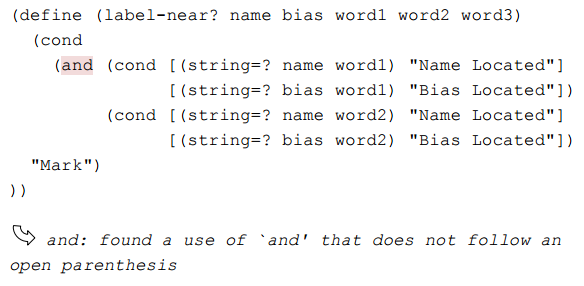
\includegraphics[keepaspectratio, width=0.5\textwidth]{MEE_example.png}
  \caption{Example of an ineffective error message in Racket}
  \label{fig:racketerrormessage}
\end{figure}

Marceau, Fisler, and Krishnamurthi grouped messages into nine most common error categories in their results from the study.
Their rubric found the level of severity of the error messages.
Through their data collection at the end of the study, they also found the level of occurrence of each error type from each lab and which error messages were poorly responded to, indicated as \textit{\%error} and \textit{\%bad}, respectively.
\textit{\#bad} shows the level of likelihood of recurrence of the respective error message.
The values of interest are the values enclosed in a box, which are the higher level \textit{\#bad} values, as seen in figure \ref{fig:drracketstudy}. 

The authors found from the data, that students have difficulties with certain errors at different points in the course.
For example, in Lab 5 of the course, the authors found that the numerous argument count errors trace to mistakes in properly closing expressions.
The error messages that the student saw from these mistakes did not match with the actual error the student encountered with their program. 

\todo[inline, color=orange]{Rephrase paragraph}

\begin{figure}[t!]
  \centering
  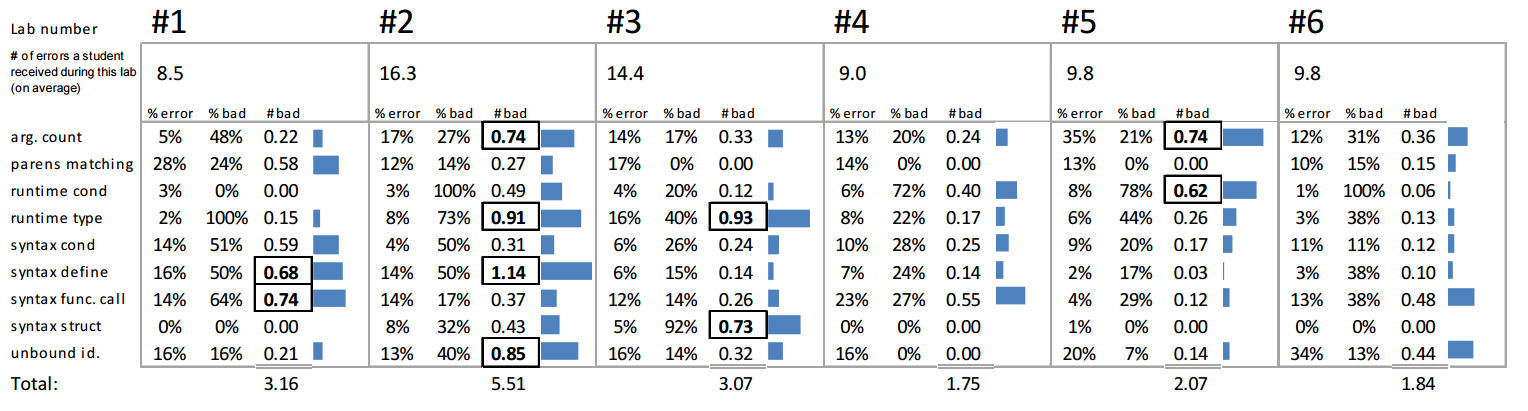
\includegraphics[keepaspectratio, width=0.5\textwidth]{MEE_Data.png}
  \caption{Results from DrRacket study}
  \label{fig:drracketstudy}
\end{figure}

\todo[inline, color=orange]{fix image positions}

\subsection{Analysis of compiler messages in C++}
Compiler error messages are often difficult to understand for many programmers, especially introductory programmers.
Not a lot of research has been conducted on compiler error message design.
In the first semester of 2002-2003, Traver conducted a case study on students' work with compiler error messages in C++ in an introductory computer science course.
The motivation of this study is to gain insight on what students are struggling with in the course and to help the professor's personal struggles with these error messages.
Traver gathered data from the students' interactions with C++ throughout the semester and wrote up analyses of the error messages received in 5 separate parts.
\begin{itemize}
	\item \textit{The error message} received from the compiler
	\item \textit{The source code} that caused the original error
	\item \textit{The diagnostic} of why the error occurred
	\item \textit{An alternate error message} that may help lead more directly to the true diagnosis of the issue.
	\item \textit{A comment} about why the error message is not helpful
\end{itemize}

Below is an example of an error message in C++ analyzed in the study along with the source code ~\cite{Traver:2010} (in the interest of space, I have not included the other parts of the analysis):

\begin{verbatim}
Source Code:

class SavingAccount 
friend ostream & operator<<
ostream &os, const SavingAccount &sA);
};
\end{verbatim}

\begin{verbatim}
Error Message:

ANSI C++ forbids declaration 
'ostream' with no type 'ostream'
is neither function nor method; 
cannot be declared friend
parse error before '&'
\end{verbatim}

In this case, the user forgot to include a header file (iostream.h), so the compiler does not know what iostream is.
The error message however, did not suggest to include a header, a simple fix, where the original error message could easily confuse novice programmers.
The author of the study noted that this type of error message should ``convey a clear message that the programmer can quickly understand and that is useful for fixing the error'', but the error message given to the user would not accomplish this for students who are still new to programming~\cite{Traver:2010}.

Traver found from the study, that there is an apparent lack of thought put into the usability of compiler error messages and that many students, especially those new to programming, will have a hard time understanding these errors.
There was no quantitative data gathered on these error messages, but rather just a general observation of how students struggled working with the compiler error messages.
Traver also noted that ``better [error messages] are possible'' and was able to provide alternative error messages for each of the ones analyzed ~\cite{Traver:2010}.
So, better error message design is possible, such that more efforts and time are put into compiler error message research. 

\section{Methodologies}
In this section, we will be discussing three tools and methodologies meant to attempt to improve the usability of error messages or suggest improvements for error message design based on the results of the analyses discussed in section 3.
The first methodology we will discuss is a set of recommendations for improving the usability of error messages.
The second approach discusses improving compiler error messages through a set of principles meant to increase usability of the messages.
For the third approach, we will discuss an attempt on enhancing syntax error messages in Java and the how well these syntax error messages improve over the original. 

\subsection{Recommendations for error messages}
This will use my source, Mind Your Language: On Novices' Interactions 
\todo[inline, color=red]{TODO}

\subsection{Principles of compiler error design}
This will use my source, On Compiler Error Messages: What They Say and What They Mean
\todo[inline, color=red]{TODO}

\subsection{Syntax error message enhancement and results}
This will use my source, Enhancing Syntax Error Messages Appears Ineffectual
\todo[inline, color=red]{TODO}


\section{Conclusion}
Discussion of the direction usability of error messages will be taken and how the methodologies will be applied for future work.

\todo[inline, color=red]{TODO}


\section{Acknowledgments}

\todo[inline, color=red]{TODO}


% The following two commands are all you need in the
% initial runs of your .tex file to
% produce the bibliography for the citations in your paper.
\bibliographystyle{acm}
% sample_paper.bib is the name of the BibTex file containing the
% bibliography entries. Note that you *don't* include the .bib ending here.
\bibliography{Usability_of_Error_Messages_for_Novice_Programmers}  

\todo[inline, color=blue]{Citing sources for references}
~\cite{Denny:2014:ESE:2591708.2591748}
~\cite{Hartmann:2010:OPS:1753326.1753478}
~\cite{Isa:1983:MOE:800045.801583}
~\cite{Kummerfeld:2003:NBF:858403.858416}
~\cite{Marceau:2011:MEE:1953163.1953308}
~\cite{Marceau:2011:MYL:2048237.2048241}
~\cite{Murphy:2008:BTD:1352135.1352193}
~\cite{Traver:2010}
% You must have a proper ".bib" file
%  and remember to run:
% latex bibtex latex latex
% to resolve all references

\end{document}
